\documentclass{standalone}
\usepackage{tikz}
\usetikzlibrary{patterns, positioning}

\begin{document}
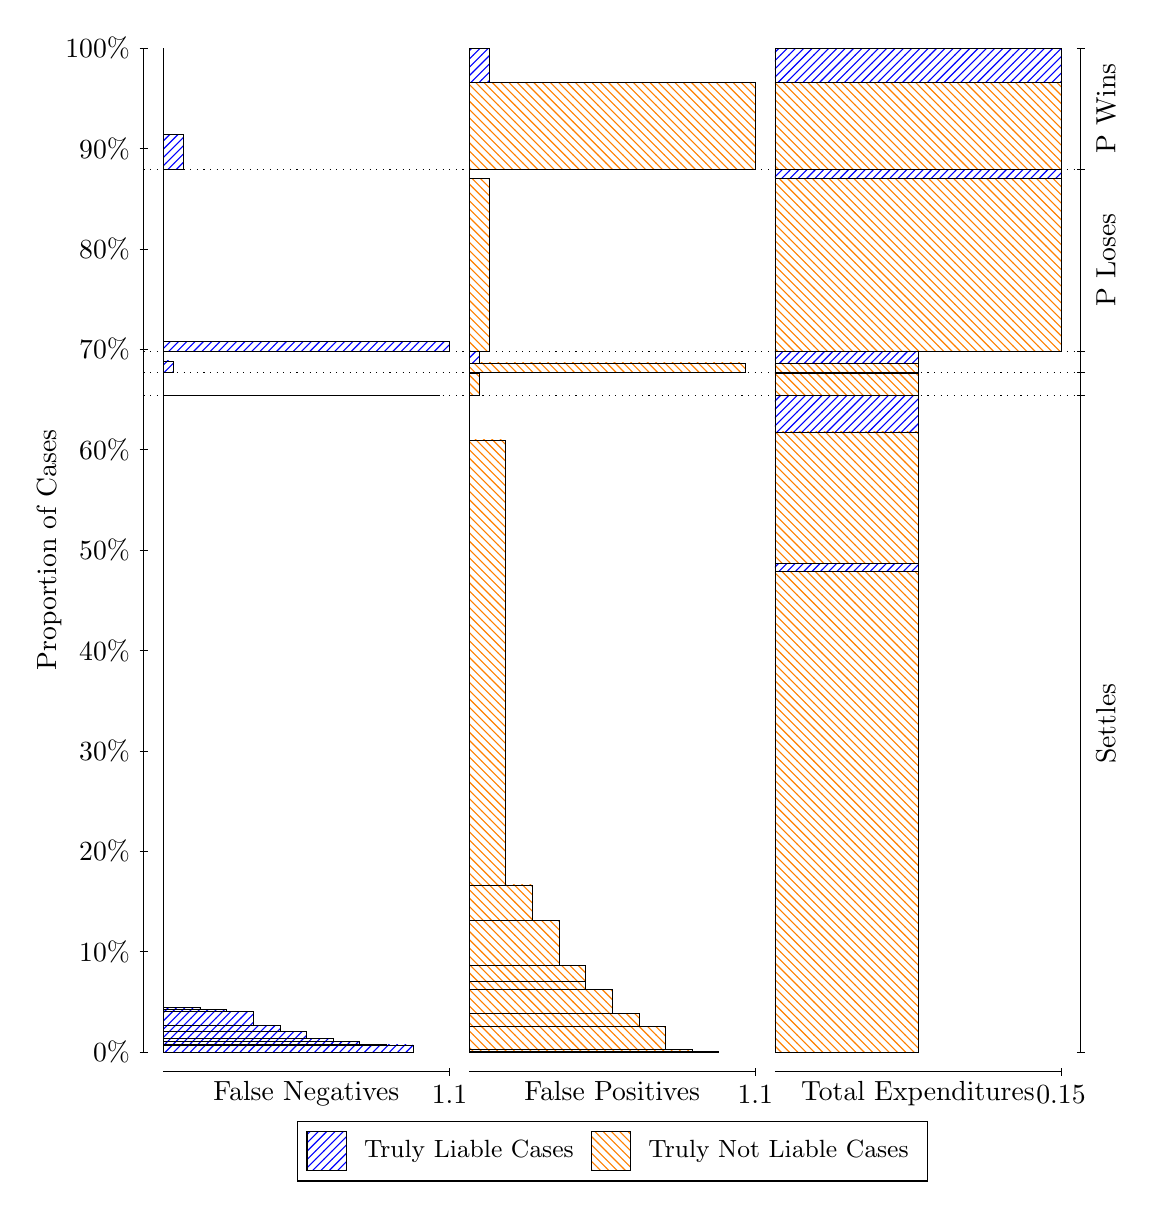
\begin{tikzpicture}
\draw[black, very thin] (1.5,1.75) -- (1.5,14.5);
\node[rotate=90, anchor=center] at (0.3, 8.125) {Proportion of Cases};
\draw[black, very thin] (1.45,1.75) -- (1.55,1.75);
\node[anchor=east] at (1.45, 1.75) {0\%};
\draw[black, very thin] (1.45,3.025) -- (1.55,3.025);
\node[anchor=east] at (1.45, 3.025) {10\%};
\draw[black, very thin] (1.45,4.3) -- (1.55,4.3);
\node[anchor=east] at (1.45, 4.3) {20\%};
\draw[black, very thin] (1.45,5.575) -- (1.55,5.575);
\node[anchor=east] at (1.45, 5.575) {30\%};
\draw[black, very thin] (1.45,6.85) -- (1.55,6.85);
\node[anchor=east] at (1.45, 6.85) {40\%};
\draw[black, very thin] (1.45,8.125) -- (1.55,8.125);
\node[anchor=east] at (1.45, 8.125) {50\%};
\draw[black, very thin] (1.45,9.4) -- (1.55,9.4);
\node[anchor=east] at (1.45, 9.4) {60\%};
\draw[black, very thin] (1.45,10.675) -- (1.55,10.675);
\node[anchor=east] at (1.45, 10.675) {70\%};
\draw[black, very thin] (1.45,11.95) -- (1.55,11.95);
\node[anchor=east] at (1.45, 11.95) {80\%};
\draw[black, very thin] (1.45,13.225) -- (1.55,13.225);
\node[anchor=east] at (1.45, 13.225) {90\%};
\draw[black, very thin] (1.45,14.5) -- (1.55,14.5);
\node[anchor=east] at (1.45, 14.5) {100\%};

\draw[black, very thin] (13.4,1.75) -- (13.4,14.5);
\draw[black, very thin] (13.35,1.75) -- (13.45,1.75);
\node[anchor=west] at (13.35, 1.75) {};
\draw[black, very thin] (13.35,10.087) -- (13.45,10.087);
\node[anchor=west] at (13.35, 10.087) {};
\draw[black, very thin] (13.35,10.378) -- (13.45,10.378);
\node[anchor=west] at (13.35, 10.378) {};
\draw[black, very thin] (13.35,10.65) -- (13.45,10.65);
\node[anchor=west] at (13.35, 10.65) {};
\draw[black, very thin] (13.35,12.962) -- (13.45,12.962);
\node[anchor=west] at (13.35, 12.962) {};
\draw[black, very thin] (13.35,14.5) -- (13.45,14.5);
\node[anchor=west] at (13.35, 14.5) {};

\draw[black, very thin, pattern color=blue, pattern=north east lines] (1.75,1.75) rectangle (4.9186,1.8391);
\draw[black, very thin, pattern color=blue, pattern=north east lines] (1.75,1.8391) rectangle (4.5806,1.8509);
\draw[black, very thin, pattern color=blue, pattern=north east lines] (1.75,1.8509) rectangle (4.2426,1.8838);
\draw[black, very thin, pattern color=blue, pattern=north east lines] (1.75,1.8838) rectangle (3.9047,1.9186);
\draw[black, very thin, pattern color=blue, pattern=north east lines] (1.75,1.9186) rectangle (3.5667,2.0072);
\draw[black, very thin, pattern color=blue, pattern=north east lines] (1.75,2.0072) rectangle (3.2287,2.086);
\draw[black, very thin, pattern color=blue, pattern=north east lines] (1.75,2.086) rectangle (2.8907,2.2702);
\draw[black, very thin, pattern color=blue, pattern=north east lines] (1.75,2.2702) rectangle (2.5527,2.295);
\draw[black, very thin, pattern color=blue, pattern=north east lines] (1.75,2.295) rectangle (2.2147,2.3134);
\draw[black, very thin, pattern color=orange, pattern=north west lines] (1.75,2.3134) rectangle (1.75,10.087);
\draw[black, very thin, pattern color=blue, pattern=north east lines] (1.75,10.087) rectangle (5.2566,10.093);
\draw[black, very thin, pattern color=orange, pattern=north west lines] (1.75,10.093) rectangle (1.75,10.378);
\draw[black, very thin, pattern color=blue, pattern=north east lines] (1.75,10.378) rectangle (1.8767,10.527);
\draw[black, very thin, pattern color=orange, pattern=north west lines] (1.75,10.527) rectangle (1.75,10.65);
\draw[black, very thin, pattern color=blue, pattern=north east lines] (1.75,10.65) rectangle (5.3833,10.771);
\draw[black, very thin, pattern color=orange, pattern=north west lines] (1.75,10.771) rectangle (1.75,12.962);
\draw[black, very thin, pattern color=blue, pattern=north east lines] (1.75,12.962) rectangle (2.0035,13.399);
\draw[black, very thin, pattern color=orange, pattern=north west lines] (1.75,13.399) rectangle (1.75,14.5);
\draw[black, very thin, pattern color=orange, pattern=north west lines] (5.6333,1.75) rectangle (8.8019,1.7623);
\draw[black, very thin, pattern color=orange, pattern=north west lines] (5.6333,1.7623) rectangle (8.464,1.7861);
\draw[black, very thin, pattern color=orange, pattern=north west lines] (5.6333,1.7861) rectangle (8.126,2.073);
\draw[black, very thin, pattern color=orange, pattern=north west lines] (5.6333,2.073) rectangle (7.788,2.2438);
\draw[black, very thin, pattern color=orange, pattern=north west lines] (5.6333,2.2438) rectangle (7.45,2.5475);
\draw[black, very thin, pattern color=orange, pattern=north west lines] (5.6333,2.5475) rectangle (7.112,2.6485);
\draw[black, very thin, pattern color=orange, pattern=north west lines] (5.6333,2.6485) rectangle (7.112,2.8496);
\draw[black, very thin, pattern color=orange, pattern=north west lines] (5.6333,2.8496) rectangle (6.774,3.4216);
\draw[black, very thin, pattern color=orange, pattern=north west lines] (5.6333,3.4216) rectangle (6.436,3.8729);
\draw[black, very thin, pattern color=orange, pattern=north west lines] (5.6333,3.8729) rectangle (6.0981,9.5238);
\draw[black, very thin, pattern color=blue, pattern=north east lines] (5.6333,9.5238) rectangle (5.6333,10.087);
\draw[black, very thin, pattern color=orange, pattern=north west lines] (5.6333,10.087) rectangle (5.7601,10.373);
\draw[black, very thin, pattern color=blue, pattern=north east lines] (5.6333,10.373) rectangle (5.6333,10.378);
\draw[black, very thin, pattern color=orange, pattern=north west lines] (5.6333,10.378) rectangle (9.1399,10.502);
\draw[black, very thin, pattern color=blue, pattern=north east lines] (5.6333,10.502) rectangle (5.7601,10.65);
\draw[black, very thin, pattern color=orange, pattern=north west lines] (5.6333,10.65) rectangle (5.8868,12.841);
\draw[black, very thin, pattern color=blue, pattern=north east lines] (5.6333,12.841) rectangle (5.6333,12.962);
\draw[black, very thin, pattern color=orange, pattern=north west lines] (5.6333,12.962) rectangle (9.2667,14.064);
\draw[black, very thin, pattern color=blue, pattern=north east lines] (5.6333,14.064) rectangle (5.8868,14.5);
\draw[black, very thin, pattern color=orange, pattern=north west lines] (9.5167,1.75) rectangle (11.333,7.8522);
\draw[black, very thin, pattern color=blue, pattern=north east lines] (9.5167,7.8522) rectangle (11.333,7.9531);
\draw[black, very thin, pattern color=orange, pattern=north west lines] (9.5167,7.9531) rectangle (11.333,9.6247);
\draw[black, very thin, pattern color=blue, pattern=north east lines] (9.5167,9.6247) rectangle (11.333,10.087);
\draw[black, very thin, pattern color=orange, pattern=north west lines] (9.5167,10.087) rectangle (11.333,10.373);
\draw[black, very thin, pattern color=blue, pattern=north east lines] (9.5167,10.373) rectangle (11.333,10.378);
\draw[black, very thin, pattern color=orange, pattern=north west lines] (9.5167,10.378) rectangle (11.333,10.502);
\draw[black, very thin, pattern color=blue, pattern=north east lines] (9.5167,10.502) rectangle (11.333,10.65);
\draw[black, very thin, pattern color=orange, pattern=north west lines] (9.5167,10.65) rectangle (13.15,12.841);
\draw[black, very thin, pattern color=blue, pattern=north east lines] (9.5167,12.841) rectangle (13.15,12.962);
\draw[black, very thin, pattern color=orange, pattern=north west lines] (9.5167,12.962) rectangle (13.15,14.064);
\draw[black, very thin, pattern color=blue, pattern=north east lines] (9.5167,14.064) rectangle (13.15,14.5);
\draw[black, dotted] (1.5,10.087) -- (13.4,10.087);
\draw[black, dotted] (1.5,10.378) -- (13.4,10.378);
\draw[black, dotted] (1.5,10.65) -- (13.4,10.65);
\draw[black, dotted] (1.5,12.962) -- (13.4,12.962);
\draw[black, very thin] (1.75,1.5) -- (5.3833,1.5);
\node[anchor=north] at (3.5667, 1.5) {False Negatives};
\draw[black, very thin] (5.3833,1.45) -- (5.3833,1.55);
\node[anchor=north] at (5.3833, 1.45) {1.1};

\draw[black, very thin] (5.6333,1.5) -- (9.2667,1.5);
\node[anchor=north] at (7.45, 1.5) {False Positives};
\draw[black, very thin] (9.2667,1.45) -- (9.2667,1.55);
\node[anchor=north] at (9.2667, 1.45) {1.1};

\draw[black, very thin] (9.5167,1.5) -- (13.15,1.5);
\node[anchor=north] at (11.333, 1.5) {Total Expenditures};
\draw[black, very thin] (13.15,1.45) -- (13.15,1.55);
\node[anchor=north] at (13.15, 1.45) {0.15};

\node[black, centered, rotate=90] at (13.72, 5.9186) {Settles};


\node[black, centered, rotate=90] at (13.72, 11.806) {P Loses};
\node[black, centered, rotate=90] at (13.72, 13.731) {P Wins};

\draw (7.449999999999999,1.5) node[draw=none] (baseCoordinate) {};
\begin{scope}[align=center]
        \matrix[scale=0.5, draw=black, below=0.5cm of baseCoordinate, nodes={draw}, column sep=0.1cm]{
            \node[rectangle, draw, minimum width=0.5cm, minimum height=0.5cm, pattern=north east lines, pattern color=blue] {}; &
            \node[draw=none, font=\small] (B) {Truly Liable Cases}; &
            \node[rectangle, draw, minimum width=0.5cm, minimum height=0.5cm, pattern=north west lines, pattern color=orange] {}; &
            \node[draw=none, font=\small] (B) {Truly Not Liable Cases}; \\
            };
\end{scope}

\end{tikzpicture}
\end{document}